\documentclass[12pt,a4paper]{article}

\usepackage[utf8]{inputenc}
\usepackage[T1]{fontenc}
\usepackage[brazilian]{babel}
\usepackage{geometry}
\usepackage{graphicx}
\usepackage{booktabs}
\usepackage{array}
\usepackage{longtable}
\usepackage{float}
\usepackage{xcolor}
\usepackage{hyperref}

\geometry{margin=2.4cm}
\hypersetup{
    colorlinks=true,
    linkcolor=blue,
    urlcolor=blue,
    citecolor=blue
}

\title{Resultados Comparativos dos Experimentos 1, 2 e 3}
\author{NCA Optimizer Benchmark}
\date{}

\begin{document}

\maketitle

\section{Objetivo da análise}

Esta seção apresenta os resultados de três protocolos experimentais para comparação de modelos e algoritmos de otimização. O objetivo não é apenas identificar a maior métrica final, mas também avaliar o custo necessário para alcançá-la. Por isso, os resultados são analisados sob três perspectivas:

\begin{enumerate}
    \item qualidade preditiva no conjunto de teste cego, usando MCC, F1 e acurácia;
    \item custo computacional, medido pelo tempo de execução;
    \item complexidade empírica do processo de otimização, medida pelo número de treinamentos ou avaliações da função objetivo.
\end{enumerate}

O ponto mais importante da revisão foi separar as métricas. MCC e acurácia não devem ser comparadas diretamente no mesmo eixo, pois medem propriedades diferentes do classificador. Assim, o Experimento 1 é apresentado primeiro pela métrica MCC, enquanto os Experimentos 2 e 3 são apresentados pela acurácia no mesmo conjunto de teste cego.

\section{Descrição dos experimentos}

Todos os experimentos usam as mesmas sementes principais, os mesmos modelos, os mesmos otimizadores e o mesmo conjunto de teste cego. A diferença entre eles está na função de fitness usada durante a busca e no protocolo de validação.

\begin{table}[H]
\centering
\caption{Resumo dos três experimentos avaliados.}
\label{tab:experimentos}
\begin{tabular}{p{2.4cm}p{4.0cm}p{4.2cm}p{3.5cm}}
\toprule
Experimento & Protocolo & Fitness durante a otimização & Métrica principal reportada \\
\midrule
Experimento 1 & Holdout temporal 60/20/20 & $0.6 \cdot MCC + 0.4 \cdot F1$ & MCC no teste cego \\
Experimento 2 & Holdout temporal 60/20/20 & $0.4 \cdot Acc_{train} + 0.6 \cdot Acc_{val}$ & Acurácia no teste cego \\
Experimento 3 & Cross-validation temporal & média dos folds de $0.4 \cdot Acc_{train} + 0.6 \cdot Acc_{val}$ & Acurácia no teste cego \\
\bottomrule
\end{tabular}
\end{table}

O Experimento 3 corresponde ao resultado anteriormente chamado de ``Experimento 4''. Na apresentação final, a nomenclatura deve ser corrigida para evitar confusão: os resultados devem ser apresentados como Experimentos 1, 2 e 3.

\section{Visão geral dos resultados}

A Figura~\ref{fig:overview} reúne os três experimentos em uma única visualização. A primeira linha mostra o Experimento 1 em MCC. A segunda e a terceira linhas mostram os Experimentos 2 e 3 em acurácia. Essa separação evita comparar valores de natureza diferente.

\begin{figure}[H]
\centering
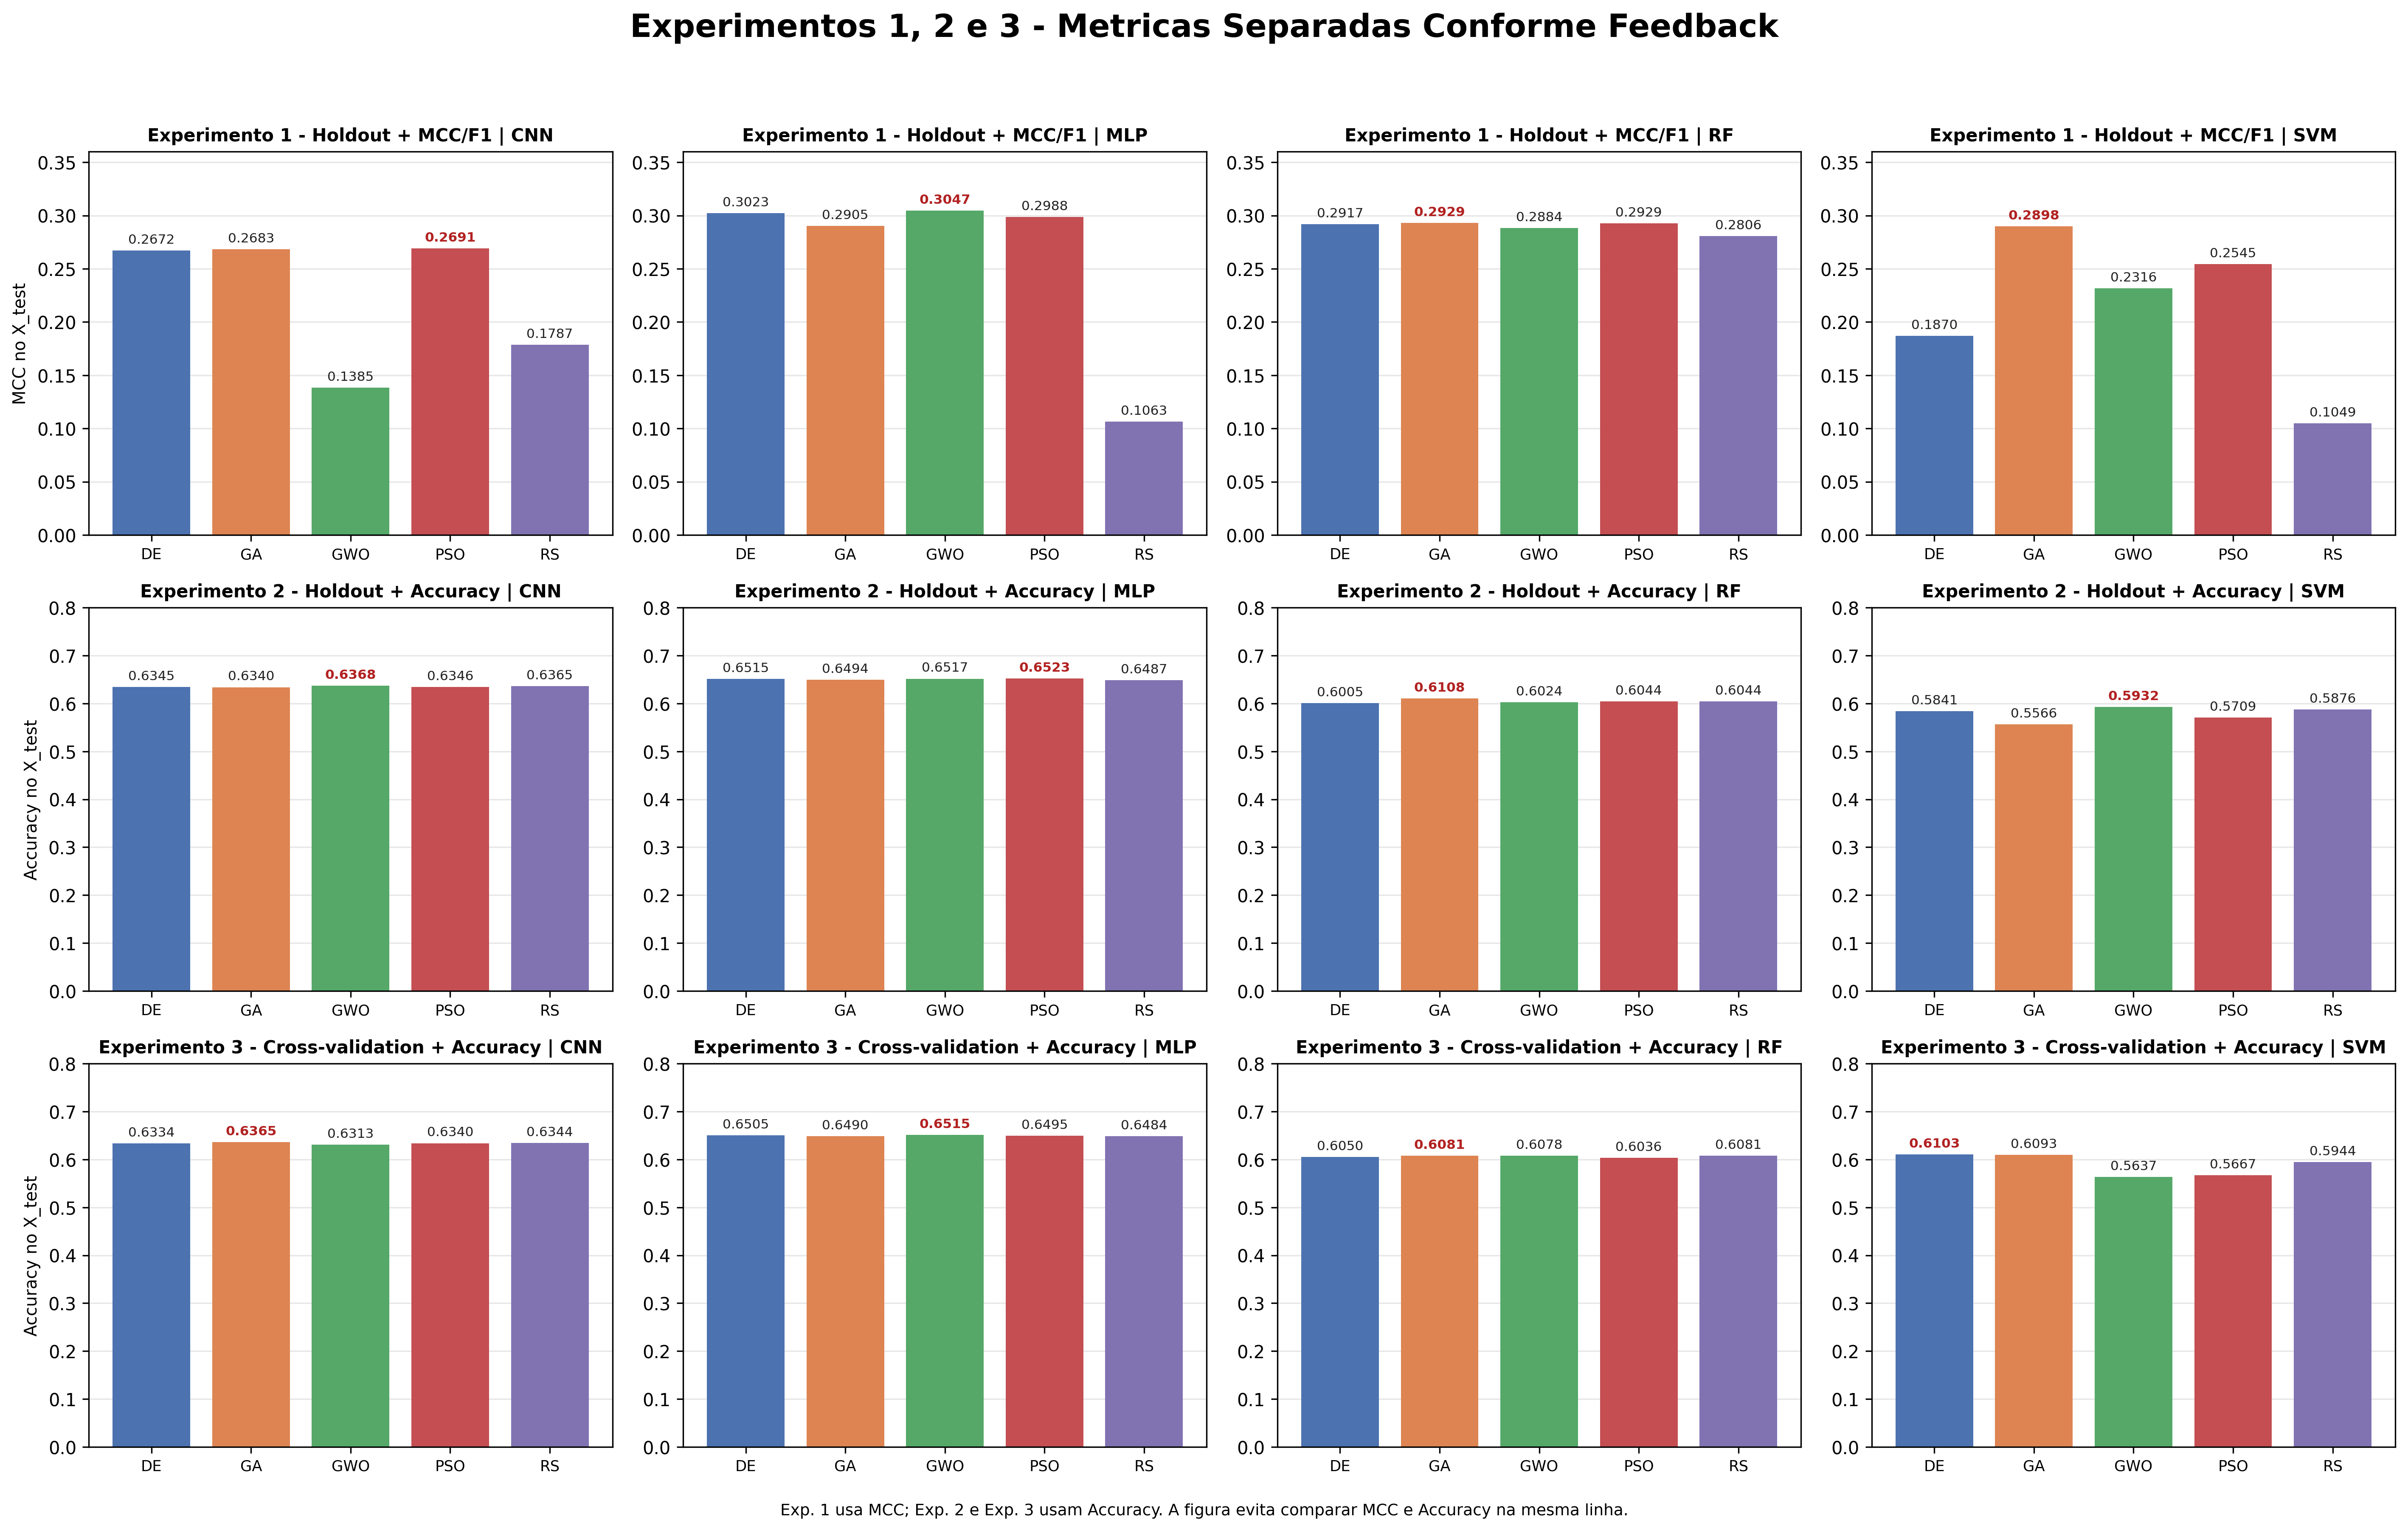
\includegraphics[width=\textwidth]{00_visao_geral_experimentos_1_2_3.png}
\caption{Visão geral dos Experimentos 1, 2 e 3. O Experimento 1 é reportado em MCC; os Experimentos 2 e 3 são reportados em acurácia.}
\label{fig:overview}
\end{figure}

A leitura principal da figura é que os melhores resultados se concentram no modelo MLP. O MLP aparece como melhor combinação nos três protocolos: MLP+GWO no Experimento 1, MLP+PSO no Experimento 2 e MLP+GWO no Experimento 3. Essa recorrência indica que o ganho não é um caso isolado de uma semente ou de um único otimizador.

\section{Experimento 1: Holdout com fitness MCC/F1}

O Experimento 1 é o protocolo mais coerente com o problema de classificação financeira, pois otimiza diretamente uma combinação de MCC e F1. O MCC é especialmente importante porque considera simultaneamente verdadeiros positivos, verdadeiros negativos, falsos positivos e falsos negativos. Assim, ele é menos vulnerável a interpretações enganosas quando a acurácia parece boa, mas o classificador erra de forma assimétrica.

\begin{figure}[H]
\centering
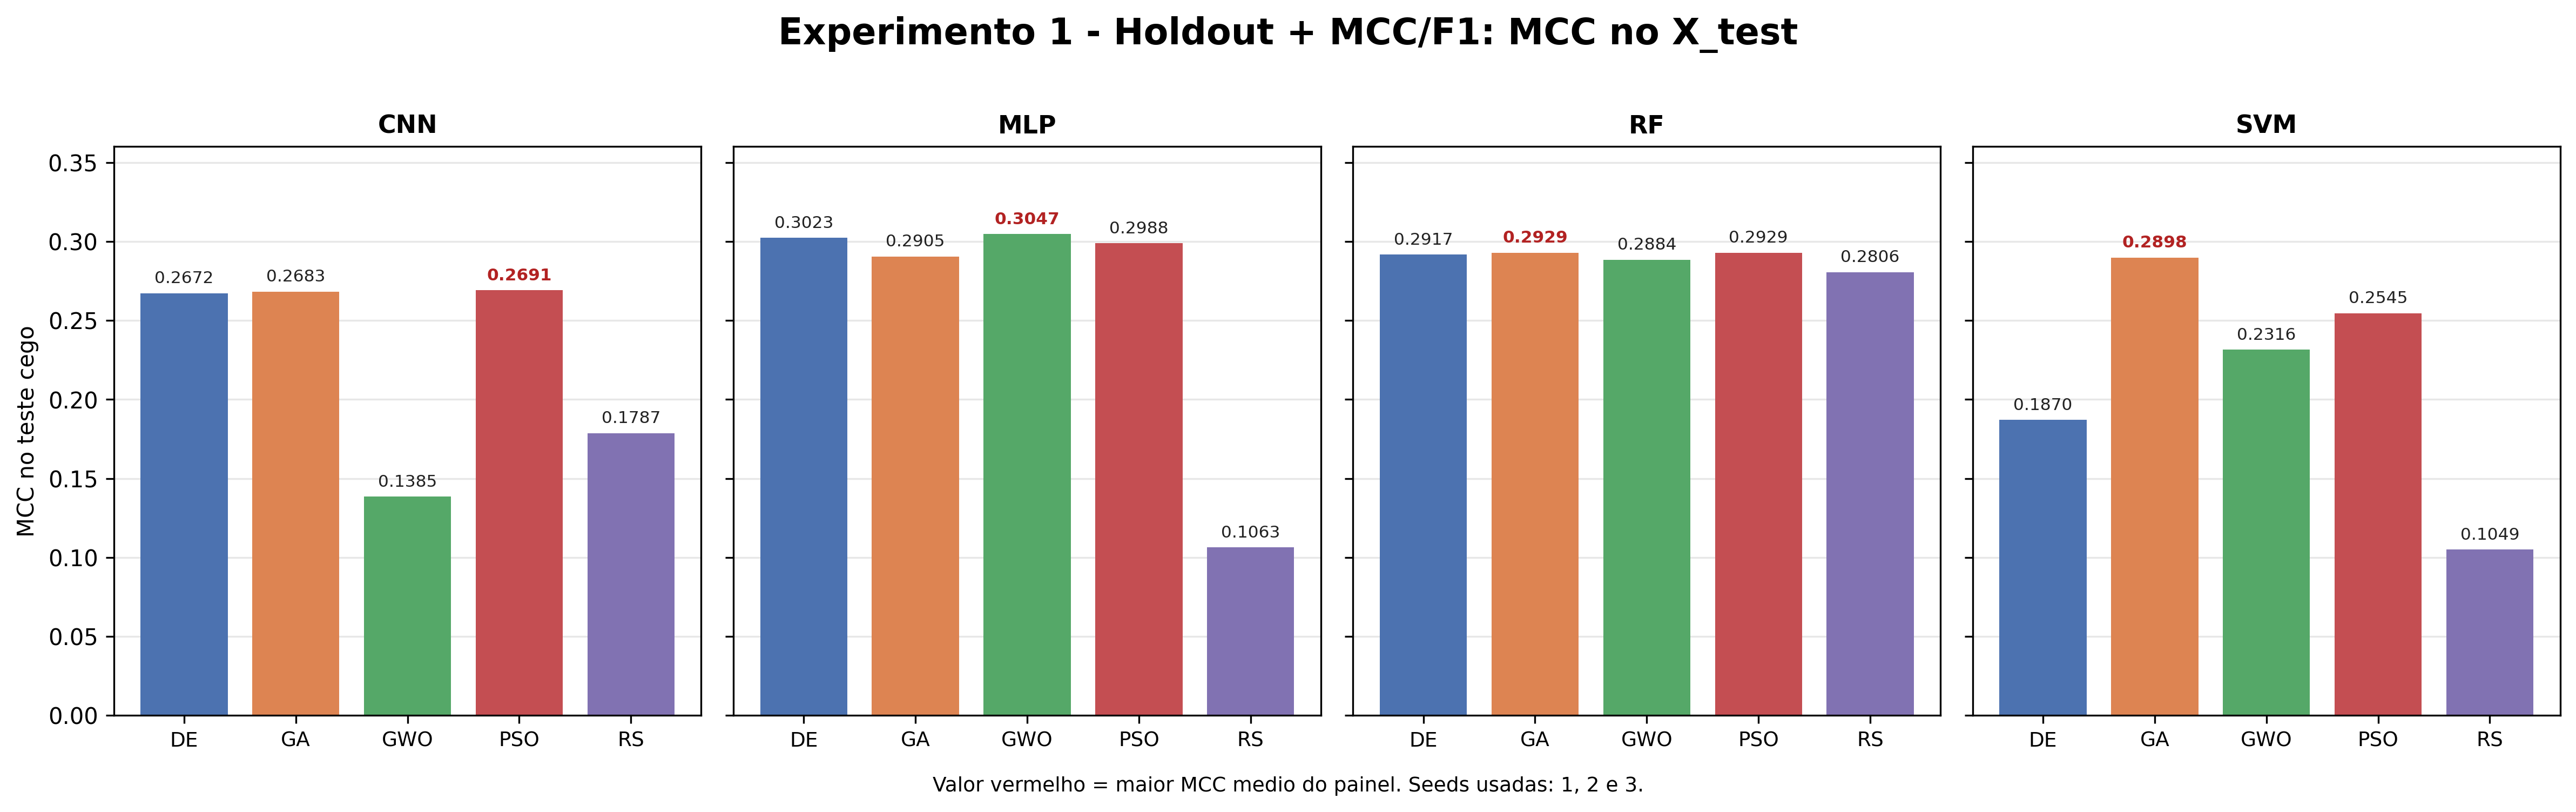
\includegraphics[width=\textwidth]{01_experimento_1_mcc_only.png}
\caption{Experimento 1 reportado somente em MCC no conjunto de teste cego.}
\label{fig:exp1_mcc}
\end{figure}

\begin{table}[H]
\centering
\caption{Melhores combinações por modelo no Experimento 1.}
\label{tab:exp1_best_model}
\small
\setlength{\tabcolsep}{4pt}
\begin{tabular}{l l r r r r r}
\toprule
Modelo & Otimizador & MCC & Acurácia & F1 & Trein. até 95\% & Min. até 95\% \\
\midrule
MLP & GWO & 0.3047 & 0.6525 & 0.6601 & 412 & 0.83 \\
RF & GA & 0.2929 & 0.6465 & 0.6694 & 595 & 13.62 \\
SVM & GA & 0.2898 & 0.6441 & 0.6770 & 780 & 143.94 \\
CNN & PSO & 0.2691 & 0.6347 & 0.6517 & 200 & 0.66 \\
\bottomrule
\end{tabular}
\end{table}

O melhor resultado absoluto do Experimento 1 foi obtido por MLP+GWO, com MCC médio de 0.3047, acurácia de 0.6525 e F1 de 0.6601. Esse é o maior MCC observado entre as combinações avaliadas e também é a maior acurácia média entre os melhores protocolos. Portanto, quando a prioridade é qualidade preditiva final, o Experimento 1 é o melhor candidato para ser tratado como protocolo principal do artigo.

Um ponto relevante é que MLP+DE ficou muito próximo do melhor resultado, com MCC de 0.3023, mas exigiu apenas 102 treinamentos para atingir 95\% do melhor fitness final, contra 412 treinamentos do MLP+GWO. Isso indica que GWO foi o melhor em desempenho absoluto, enquanto DE foi uma alternativa muito forte em custo-benefício.

\section{Experimentos 1 e 2 em acurácia no holdout}

A Figura~\ref{fig:holdout_acc} mostra a acurácia no teste cego para os dois experimentos com holdout. Essa figura responde diretamente ao pedido de reportar acurácia sem misturá-la com MCC.

\begin{figure}[H]
\centering
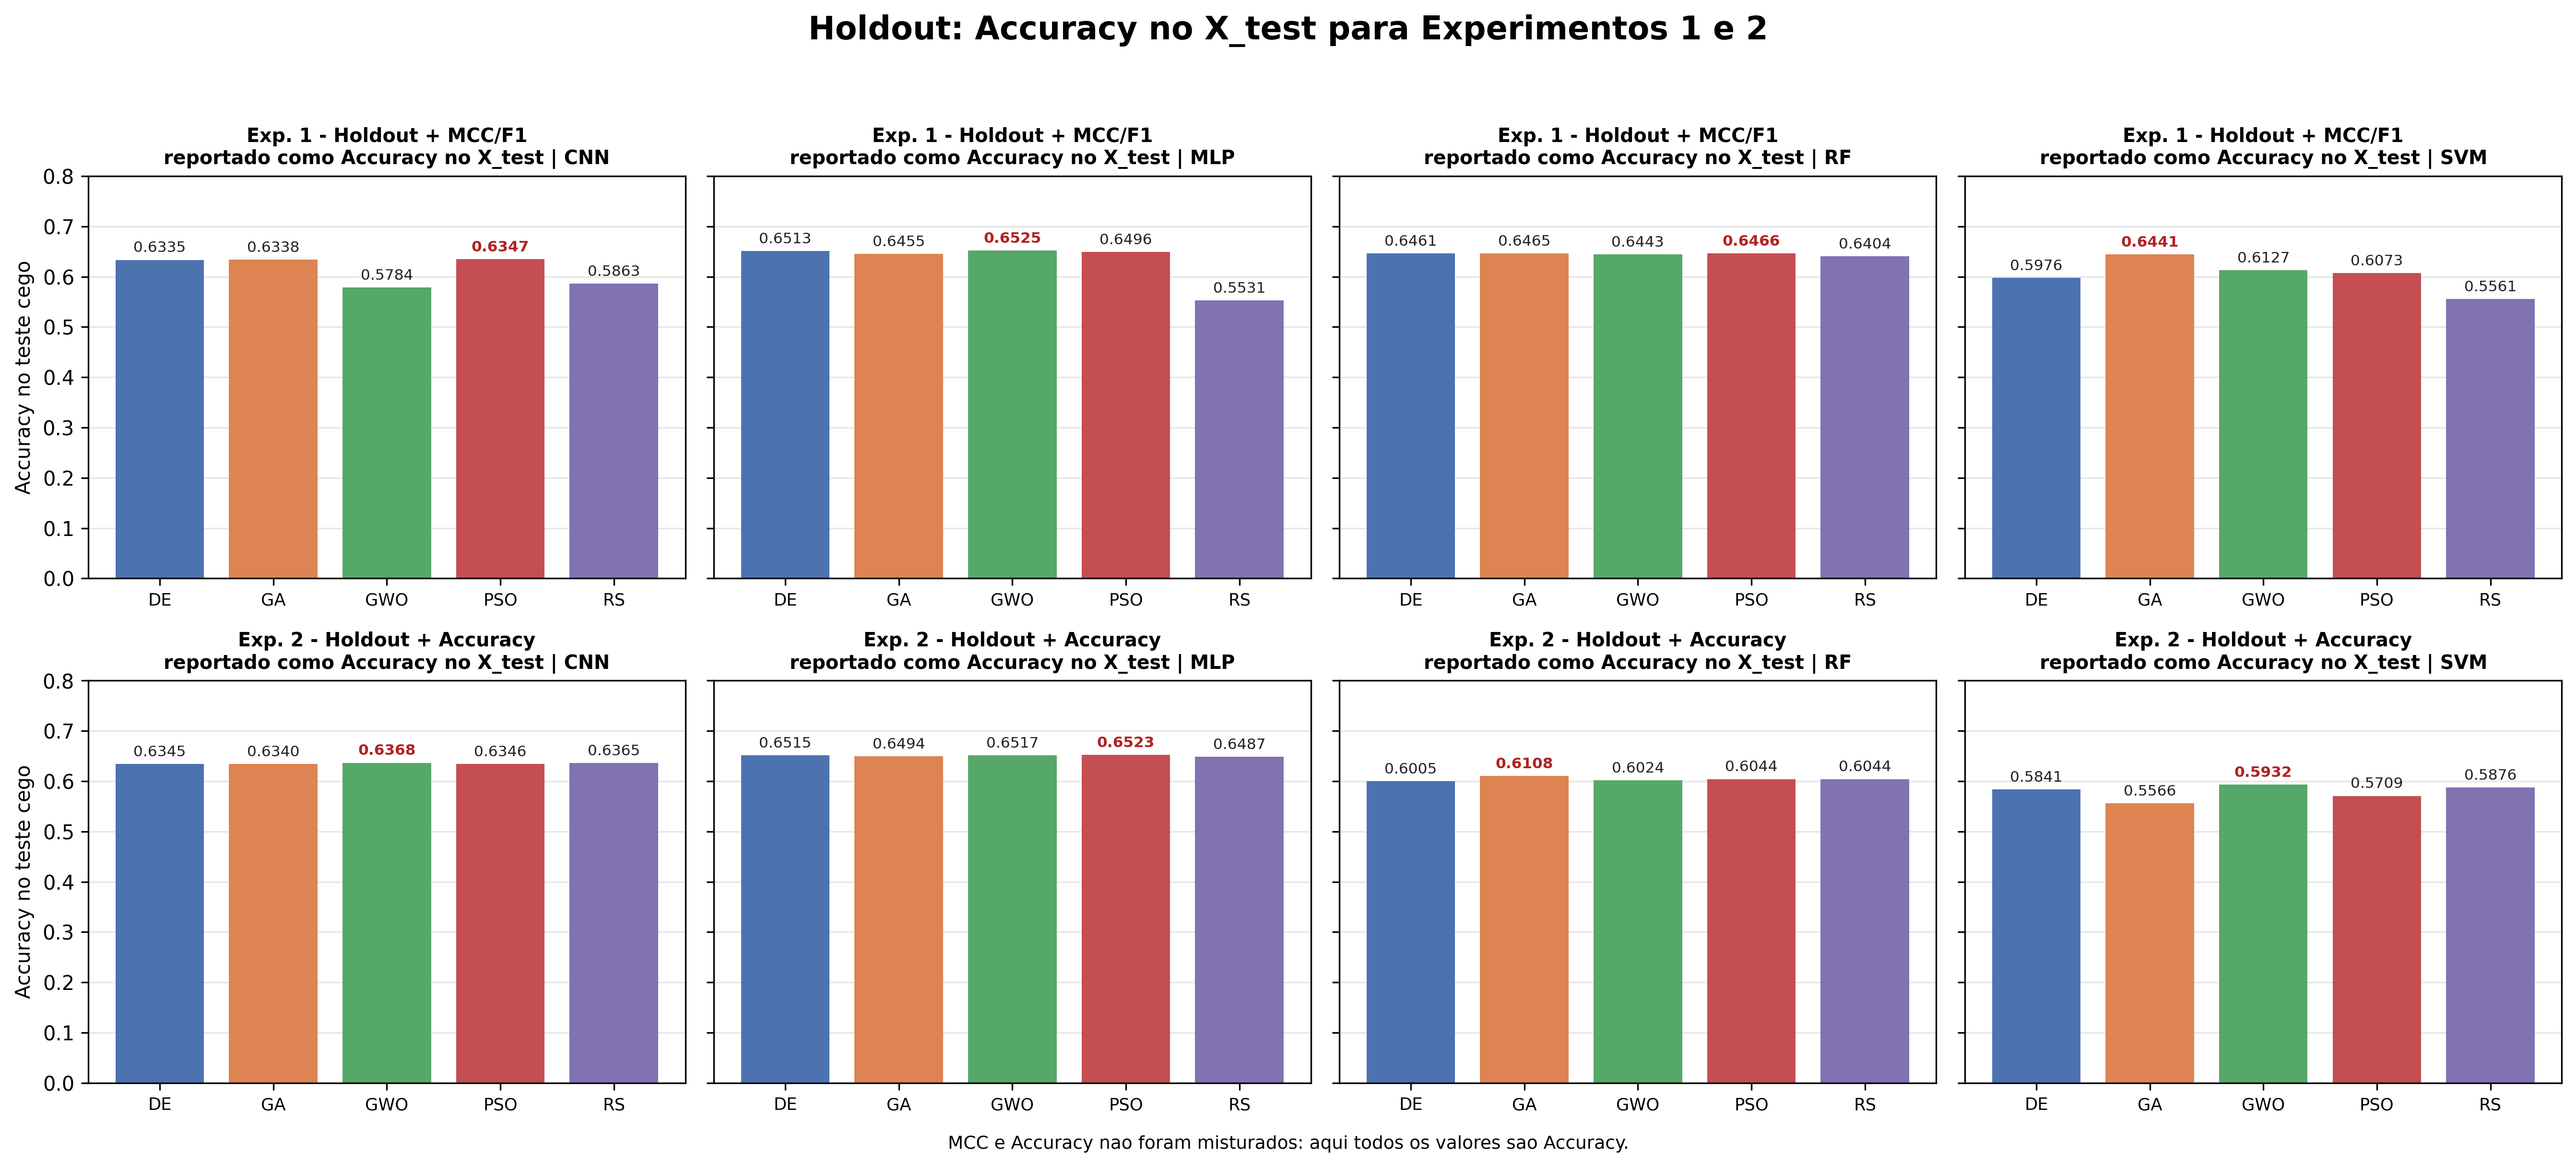
\includegraphics[width=\textwidth]{02_experimentos_1_2_holdout_accuracy.png}
\caption{Acurácia no teste cego para os Experimentos 1 e 2, ambos com protocolo holdout.}
\label{fig:holdout_acc}
\end{figure}

\begin{table}[H]
\centering
\caption{Comparação dos melhores resultados de holdout.}
\label{tab:holdout_comparison}
\small
\setlength{\tabcolsep}{4pt}
\begin{tabular}{l l l r r r r r}
\toprule
Experimento & Modelo & Otimizador & Acurácia & MCC & F1 & Trein. até 95\% & Min. até 95\% \\
\midrule
Exp. 1 & MLP & GWO & 0.6525 & 0.3047 & 0.6601 & 412 & 0.83 \\
Exp. 2 & MLP & PSO & 0.6523 & 0.3043 & 0.6586 & 114 & 0.19 \\
\bottomrule
\end{tabular}
\end{table}

Os dois resultados são muito próximos em acurácia. O Experimento 1 ainda apresenta leve vantagem: 0.6525 contra 0.6523. A diferença é pequena, mas o Experimento 1 tem uma vantagem metodológica importante: ele escolhe os hiperparâmetros com base em MCC/F1, métricas mais informativas para problemas em que a acurácia pode esconder erros relevantes. Por isso, mesmo quando olhamos para acurácia, o Experimento 1 continua competitivo.

O Experimento 2, por outro lado, mostra que a otimização direta de acurácia é mais eficiente em termos de avaliações para a melhor combinação MLP+PSO. Ele chegou a 95\% do melhor fitness em 114 treinamentos, enquanto MLP+GWO no Experimento 1 precisou de 412. Portanto, o Experimento 2 é forte como análise complementar de eficiência, mas não supera o Experimento 1 como protocolo principal.

\section{Experimento 3: Cross-validation com acurácia}

O Experimento 3 avalia a versão com validação cruzada temporal e fitness baseado em acurácia. Ele deve ser apresentado separado dos experimentos holdout, pois o protocolo de validação é diferente.

\begin{figure}[H]
\centering
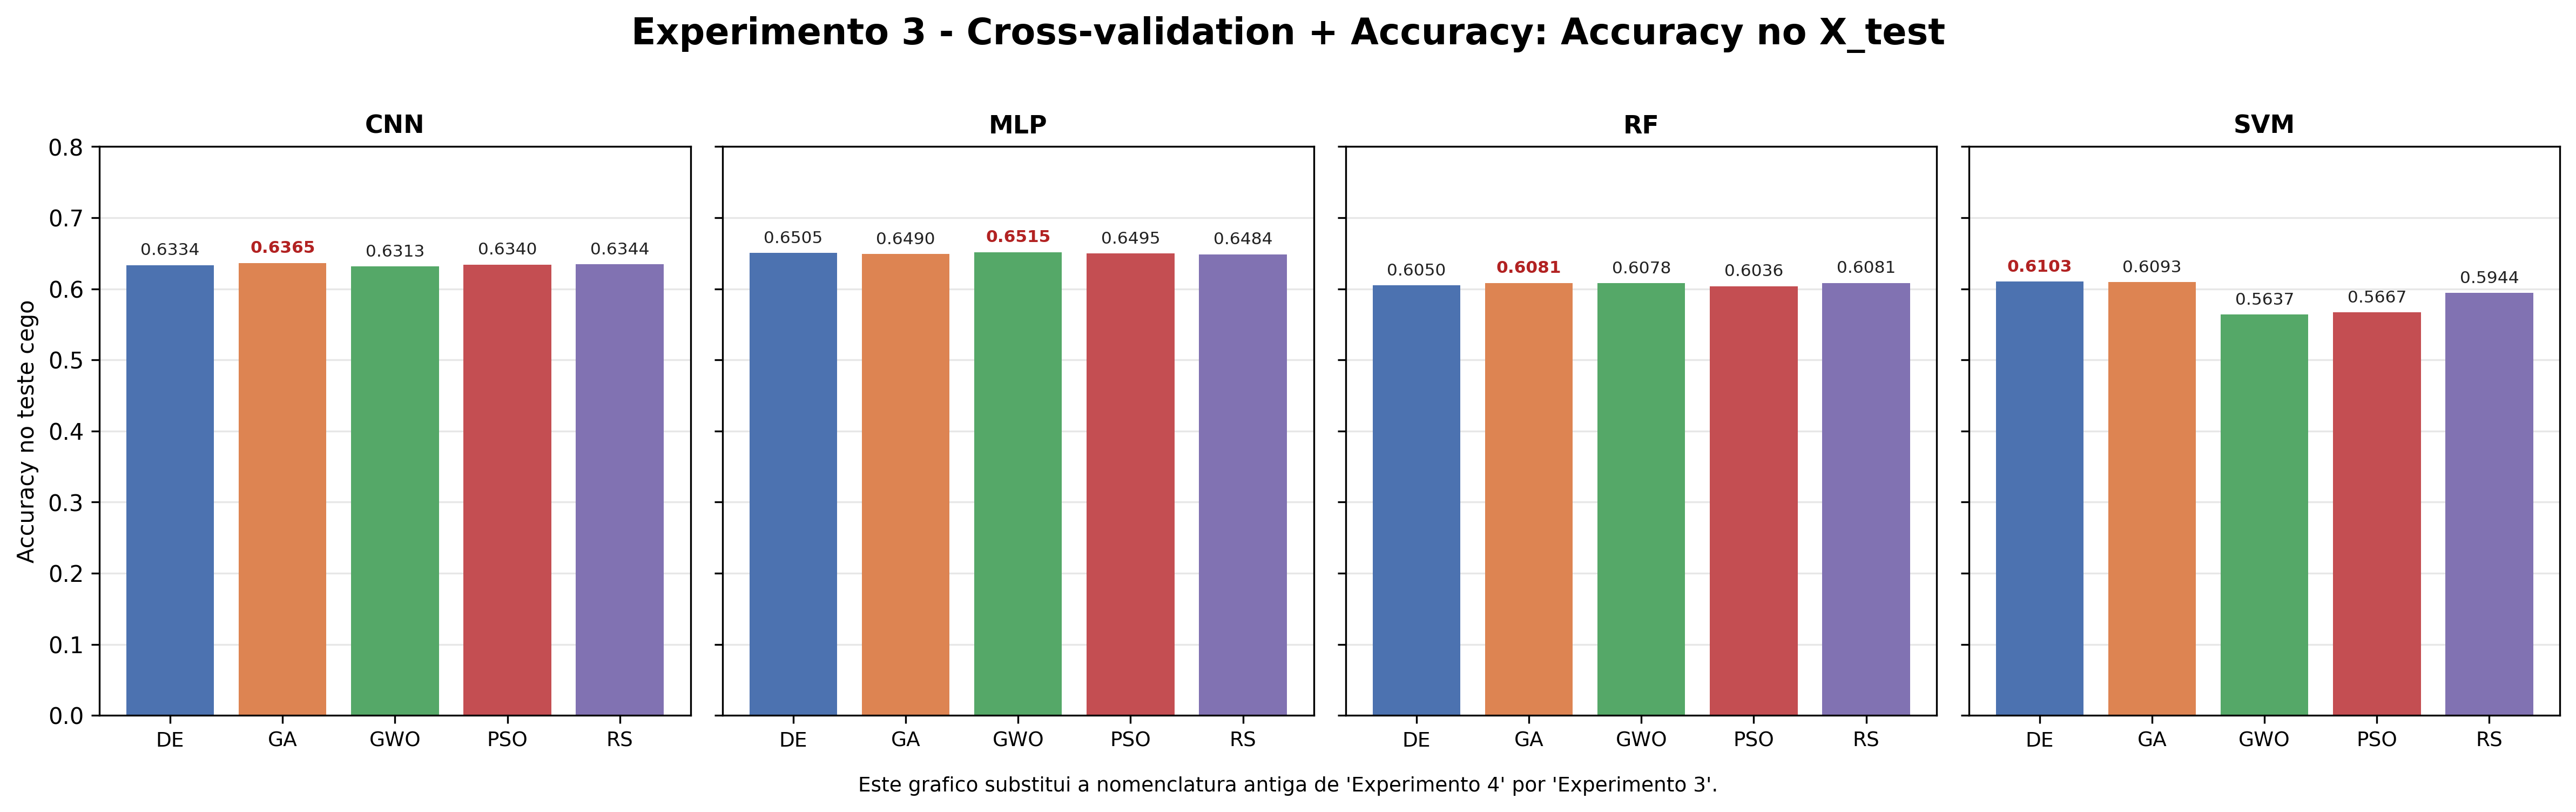
\includegraphics[width=\textwidth]{03_experimento_3_cv_accuracy_only.png}
\caption{Experimento 3 reportado separadamente: cross-validation temporal com acurácia no teste cego.}
\label{fig:exp3_cv}
\end{figure}

\begin{table}[H]
\centering
\caption{Melhores combinações por modelo no Experimento 3.}
\label{tab:exp3_best_model}
\small
\setlength{\tabcolsep}{4pt}
\begin{tabular}{l l r r r r r}
\toprule
Modelo & Otimizador & Acurácia & MCC & F1 & Trein. até 95\% & Min. até 95\% \\
\midrule
MLP & GWO & 0.6515 & 0.3028 & 0.6580 & 534 & 1.84 \\
CNN & GA & 0.6365 & 0.2726 & 0.6537 & 242 & 1.41 \\
SVM & DE & 0.6103 & 0.2205 & 0.6454 & 15 & 0.13 \\
RF & GA & 0.6081 & 0.2154 & 0.6269 & 37 & 10.04 \\
\bottomrule
\end{tabular}
\end{table}

O Experimento 3 confirma a robustez do MLP, mas não supera o Experimento 1. A melhor combinação foi MLP+GWO, com acurácia de 0.6515 e MCC de 0.3028. Esses valores são ligeiramente inferiores aos do Experimento 1. Além disso, o custo para atingir 95\% do melhor fitness foi maior: 534 treinamentos para MLP+GWO no Experimento 3, contra 412 no Experimento 1.

\section{Tempo, custo e complexidade empírica}

Para comparar algoritmos de otimização de maneira justa, não basta observar o tempo total, pois pequenas variações de hardware, paralelismo e tipo de modelo podem alterar o tempo de execução. Uma medida mais controlada é contar quantas vezes a função objetivo foi avaliada. Neste projeto, cada linha dos arquivos \texttt{*\_runs.csv} representa uma avaliação de candidato, isto é, um treinamento ou ajuste de hiperparâmetros.

A complexidade externa dos otimizadores pode ser descrita pelo número de avaliações:

\begin{table}[H]
\centering
\caption{Interpretação da complexidade externa dos otimizadores.}
\label{tab:complexity}
\small
\begin{tabular}{p{2.8cm}p{5.0cm}p{5.2cm}}
\toprule
Otimizador & Forma de contagem & Complexidade externa aproximada \\
\midrule
Random Search & número de candidatos amostrados & $O(N \cdot C_{train})$ \\
GA & população $\times$ gerações & $O(P \cdot G \cdot C_{train})$ \\
PSO & partículas $\times$ iterações & $O(P \cdot T \cdot C_{train})$ \\
DE & população $\times$ gerações & $O(P \cdot G \cdot C_{train})$ \\
GWO & lobos $\times$ iterações & $O(W \cdot T \cdot C_{train})$ \\
\bottomrule
\end{tabular}
\end{table}

Como o orçamento máximo foi controlado, o diferencial passa a ser quantas avaliações são necessárias para chegar perto do melhor resultado. A Figura~\ref{fig:effort} mostra a mediana de treinamentos necessários para atingir 95\% do melhor fitness final.

\begin{figure}[H]
\centering
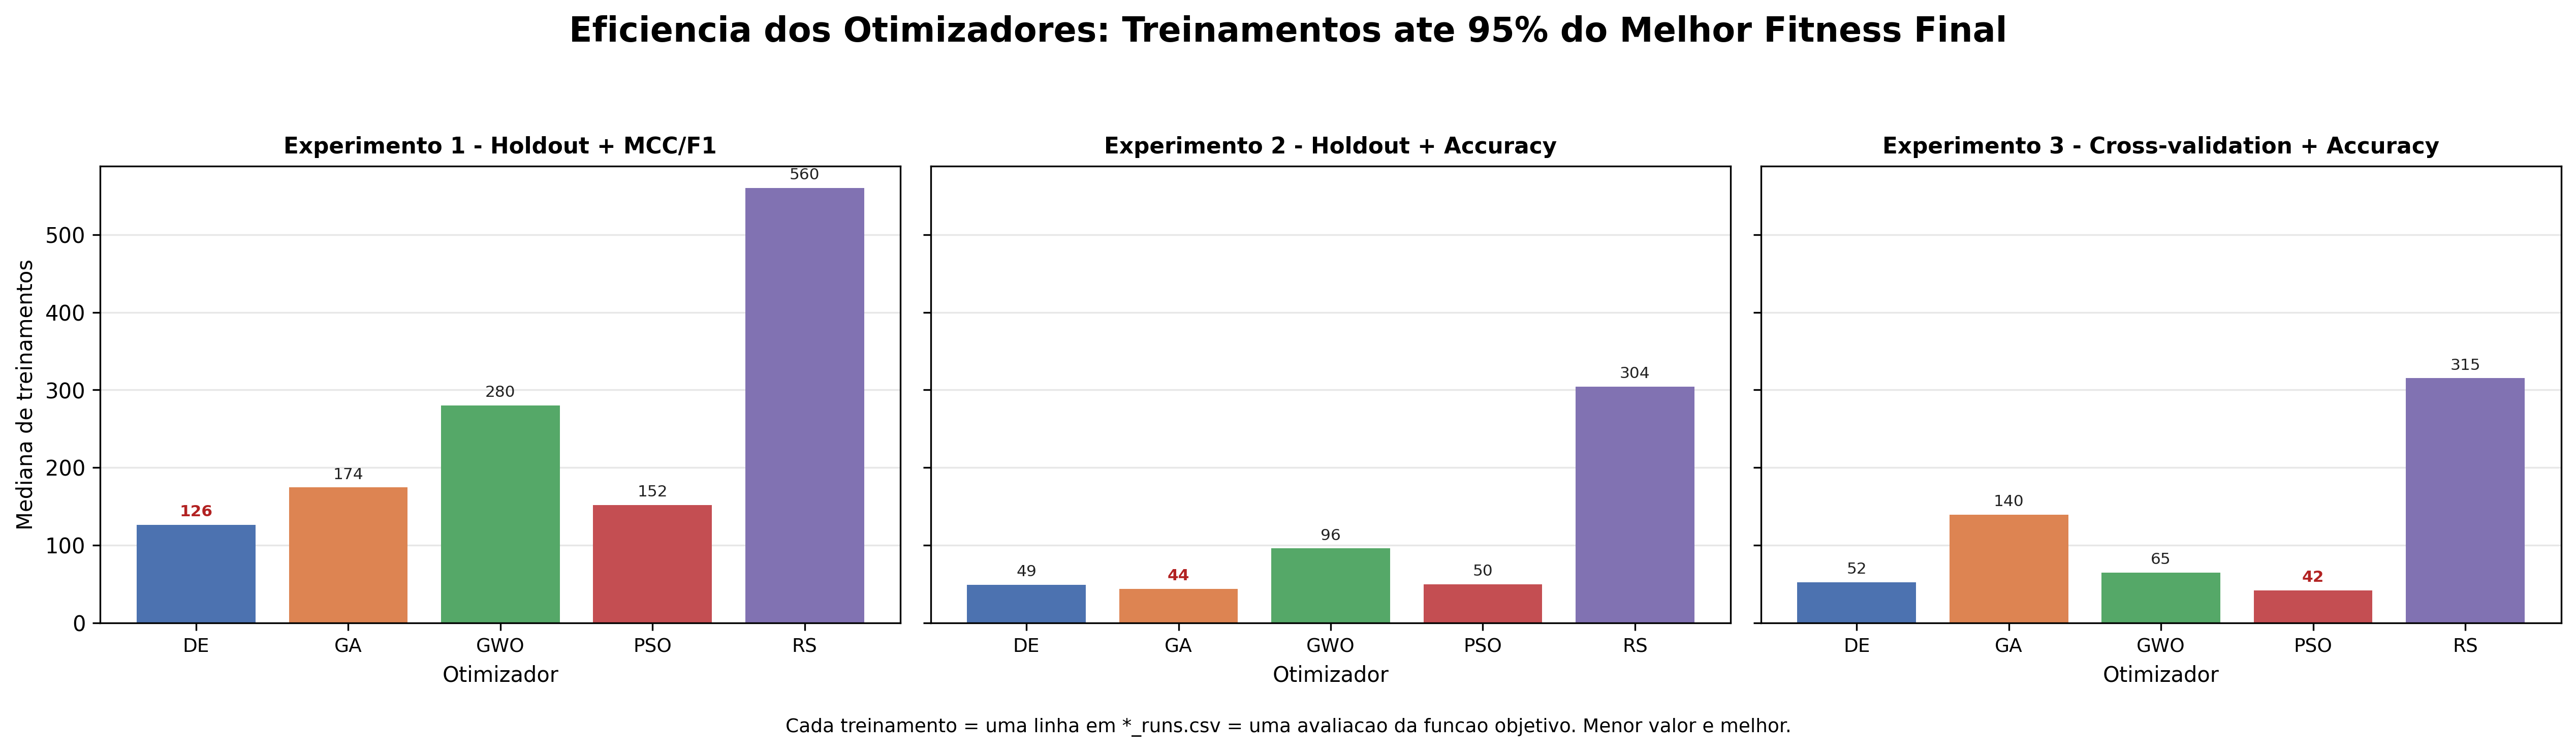
\includegraphics[width=\textwidth]{04_treinamentos_ate_bom_resultado_exp1_exp2_exp3.png}
\caption{Número mediano de treinamentos necessários para atingir 95\% do melhor fitness final em cada experimento.}
\label{fig:effort}
\end{figure}

\begin{table}[H]
\centering
\caption{Custo mediano por otimizador em cada experimento.}
\label{tab:effort_optimizer}
\small
\setlength{\tabcolsep}{4pt}
\begin{tabular}{l l r r r}
\toprule
Experimento & Otimizador & Trein. até 95\% & Min. até 95\% & Runtime total mediano \\
\midrule
Exp. 1 & DE & 126.5 & 0.66 & 4.27 \\
Exp. 1 & GA & 317.0 & 6.84 & 22.69 \\
Exp. 1 & GWO & 261.5 & 1.18 & 4.80 \\
Exp. 1 & PSO & 171.0 & 3.13 & 22.68 \\
Exp. 1 & RS & 560.0 & 28.51 & 45.09 \\
\midrule
Exp. 2 & DE & 63.0 & 0.24 & 4.15 \\
Exp. 2 & GA & 44.0 & 0.65 & 6.95 \\
Exp. 2 & GWO & 136.3 & 0.56 & 4.76 \\
Exp. 2 & PSO & 50.0 & 0.27 & 5.75 \\
Exp. 2 & RS & 162.0 & 1.49 & 4.23 \\
\midrule
Exp. 3 & DE & 58.0 & 0.59 & 7.68 \\
Exp. 3 & GA & 139.5 & 3.20 & 10.37 \\
Exp. 3 & GWO & 98.8 & 1.80 & 9.89 \\
Exp. 3 & PSO & 42.0 & 0.33 & 10.97 \\
Exp. 3 & RS & 201.0 & 4.30 & 7.98 \\
\bottomrule
\end{tabular}
\end{table}

Essa análise mostra que Random Search foi, em geral, o menos eficiente em número de avaliações. Ele pode encontrar bons candidatos, mas precisa de mais tentativas para se aproximar do melhor resultado. Em contraste, DE, GA e PSO frequentemente chegam mais cedo a uma região de boa solução. No Experimento 1, DE teve o menor custo mediano até 95\% do melhor fitness. No Experimento 2, GA teve o menor número de treinamentos. No Experimento 3, PSO foi o mais rápido em número de treinamentos.

\section{Síntese dos vencedores}

\begin{table}[H]
\centering
\caption{Resumo dos vencedores por critério.}
\label{tab:winners}
\begin{tabular}{p{4.2cm}p{4.2cm}p{6.2cm}}
\toprule
Critério & Vencedor & Justificativa \\
\midrule
Melhor experimento geral & Experimento 1 & Maior MCC observado, maior acurácia entre os melhores resultados e fitness mais adequado ao problema. \\
Melhor modelo & MLP & Aparece como melhor modelo nos três experimentos e mantém baixo tempo de execução. \\
Melhor otimizador em desempenho final & GWO & Vence no Experimento 1 em MCC e no Experimento 3 em acurácia, ambos com MLP. \\
Melhor combinação absoluta & Experimento 1 + MLP + GWO & MCC 0.3047, acurácia 0.6525 e F1 0.6601 no teste cego. \\
Melhor custo-benefício no Experimento 1 & MLP + DE & MCC 0.3023, muito próximo do melhor, mas com 102 treinamentos até 95\% do fitness. \\
Melhor alternativa focada em acurácia & Experimento 2 + MLP + PSO & Acurácia 0.6523 e apenas 114 treinamentos até 95\% do melhor fitness. \\
\bottomrule
\end{tabular}
\end{table}

\section{Conclusão}

O melhor experimento para ser defendido como protocolo principal é o Experimento 1, com holdout temporal e fitness MCC/F1. Ele é o mais consistente metodologicamente porque otimiza métricas mais informativas para classificação financeira e, ao mesmo tempo, entrega o melhor resultado final observado. A melhor combinação absoluta foi MLP+GWO, com MCC de 0.3047, acurácia de 0.6525 e F1 de 0.6601.

O melhor modelo foi o MLP. Ele venceu nos três experimentos quando se considera a melhor combinação por protocolo. Além disso, teve tempo de execução muito inferior ao Random Forest e ao SVM em várias combinações, especialmente quando executado com backend acelerado. Isso torna o MLP a escolha mais forte tanto em desempenho quanto em viabilidade computacional.

O melhor otimizador depende do critério usado. Se o critério principal for desempenho final, GWO é o melhor, pois produziu o melhor resultado absoluto no Experimento 1 e também o melhor resultado do Experimento 3. Se o critério incluir fortemente complexidade empírica, DE e PSO tornam-se alternativas importantes: DE chegou muito perto do melhor MCC no Experimento 1 com menos avaliações, e PSO foi o melhor no Experimento 2 em acurácia.

Portanto, a recomendação final é apresentar o Experimento 1 com MLP+GWO como resultado principal do artigo, acompanhado de uma discussão de eficiência mostrando que MLP+DE e MLP+PSO são alternativas competitivas quando o custo de otimização é priorizado. Essa forma de apresentar os resultados responde à observação do professor: quando os resultados finais são muito parecidos, o diferencial passa a ser quantos treinamentos foram necessários para chegar a bons parâmetros.

\end{document}
